\documentclass[11pt,a4paper]{article}
\usepackage[margin=24mm,headheight=15pt]{geometry}
\usepackage{fontspec}
\setmainfont{Latin Modern Roman}
\setsansfont{Latin Modern Sans}
\setmonofont{Latin Modern Mono}
\usepackage[spanish,es-tabla,es-nolists,es-lcroman]{babel}
\usepackage{amsmath,amssymb}
\usepackage{graphicx}
\usepackage{booktabs,tabularx,longtable,array}
\usepackage[table]{xcolor}
\usepackage{microtype}
\usepackage{enumitem}
\usepackage{caption}
\usepackage{xurl}
\usepackage[unicode,hidelinks]{hyperref}
\usepackage{fancyhdr}
\usepackage{titlesec}
\usepackage{needspace}
\definecolor{ink}{HTML}{243B53}
\definecolor{muted}{HTML}{526475}
\definecolor{light}{HTML}{EFF3F6}
\pagestyle{fancy}
\fancyhf{}
\fancyhead[L]{\small\sffamily\color{muted}Beyond Beta}
\fancyhead[R]{\small\sffamily\color{muted}Inversiones Financieras}
\fancyfoot[C]{\small\thepage}
\renewcommand{\headrulewidth}{0.3pt}
\setlength{\parindent}{0pt}
\setlength{\parskip}{6pt}
\setlength{\emergencystretch}{2em}
\setlength{\tabcolsep}{4pt}
\renewcommand{\arraystretch}{1.23}
\newcolumntype{L}[1]{>{\raggedright\arraybackslash}p{#1}}
\newcolumntype{Y}{>{\raggedright\arraybackslash}X}
\titleformat{\section}{\large\sffamily\bfseries\color{ink}}{\thesection}{.7em}{}
\titleformat{\subsection}{\normalsize\sffamily\bfseries\color{ink}}{\thesubsection}{.7em}{}
\titlespacing*{\section}{0pt}{14pt}{8pt}
\captionsetup{font=small,labelfont=bf,skip=6pt,hypcap=false}
\setlist[itemize]{leftmargin=1.4em,itemsep=3pt,topsep=4pt}
\setcounter{secnumdepth}{2}
\widowpenalty=10000
\clubpenalty=10000

\newcolumntype{R}[1]{>{\raggedleft\arraybackslash}p{#1}}
\makeatletter
\renewcommand*\l@section{\@dottedtocline{1}{0em}{2.7em}}
\makeatother


% ACADEMIC_FRONTMATTER
\hypersetup{pdftitle={Beyond Beta: el CAPM y los modelos multifactoriales en la práctica},
pdfauthor={Alonso Castro Freibott, Pablo Caonabo Crespo de la Cruz, Carlos Segovia Domínguez y Jaime Blanco González},
pdfsubject={Informe académico de Inversiones Financieras},pdfkeywords={CAPM, Fama-French, cartera, rentabilidad, riesgo}}
\begin{document}
\pagenumbering{gobble}
\begin{titlepage}
\thispagestyle{empty}
\vspace*{12mm}
{\sffamily\bfseries\color{ink}CUNEF Universidad\par}
\vspace{4mm}
{\sffamily\normalsize Inversiones Financieras\par}
\vspace{20mm}
{\sffamily\bfseries\fontsize{38}{44}\selectfont\color{ink}Beyond Beta\par}
\vspace{7mm}
{\sffamily\Large\color{ink}El CAPM y los modelos\par multifactoriales en la práctica\par}
\vspace{5mm}
{\large Informe académico\par}
\vspace{9mm}
{\color{ink}\rule{\linewidth}{0.8pt}\par}
\vspace{8mm}
\colorbox{light}{\parbox{\dimexpr\linewidth-2\fboxsep\relax}{\vspace{4mm}\hspace{3mm}\textbf{Periodo de análisis y moneda}\\[2mm]\hspace{3mm}octubre de 2021 a septiembre de 2026 | USD\vspace{4mm}}}\par
\vspace{8mm}
{\sffamily\bfseries\color{ink}Autores\par}\vspace{2mm}
Alonso Castro Freibott\\
Pablo Caonabo Crespo de la Cruz\\
Carlos Segovia Domínguez\\
Jaime Blanco González\par
\vspace{7mm}
{\sffamily\bfseries\color{ink}Profesor\par}
Javier Fernández Sánchez de la Viña\par
\vfill
{\small Curso académico 2026--2027\hfill Noviembre de 2026\par}
\end{titlepage}
\pagenumbering{roman}
\setcounter{tocdepth}{2}
\renewcommand{\contentsname}{Índice de contenidos}
\renewcommand{\listfigurename}{Índice de figuras}
\renewcommand{\listtablename}{Índice de tablas}
\renewcommand{\tablename}{Tabla}
\tableofcontents
\clearpage
\phantomsection
\addcontentsline{toc}{section}{Índice de figuras}
\listoffigures
\vspace{10mm}
\phantomsection
\addcontentsline{toc}{section}{Índice de tablas}
\listoftables
\clearpage
\pagenumbering{arabic}
\section{Resumen ejecutivo}
Comparamos la rentabilidad y el riesgo de 6 activos. El análisis pregunta qué proporción de la variación de sus excesos de rentabilidad mensual explica el mercado estadounidense y si añadir tamaño y valor mejora el ajuste para la cartera. La muestra contiene 61 precios (septiembre de 2021 a septiembre de 2026) y 60 rentabilidades mensuales (octubre de 2021 a septiembre de 2026). Las regresiones se estiman en USD y las estadísticas descriptivas también se presentan en EUR.

La cartera acumuló un 42,30 \%. Su rentabilidad geométrica anualizada fue del 7,31 \% y su volatilidad anualizada, del 17,91 \%. La mayor caída entre cierres mensuales fue del 31,88 \% desde un máximo previo.

En la cartera, R\textsuperscript{2} pasa de 0,4969 a 0,5110, mientras R\textsuperscript{2} ajustado pasa de 0,4882 a 0,4848. El incremento de ajuste bruto es pequeño frente a los dos regresores adicionales.

\Needspace{7\baselineskip}\section{Datos y decisión de moneda}
\begin{equation*}
P^{\mathrm{USD}}_{i,t}=P^{\mathrm{EUR}}_{i,t}X_{i,t},\qquad X_{i,t}=\text{USD por EUR en la fecha usada para el activo }i.
\end{equation*}
La selección ilustrativa combina tres acciones individuales con oro físico, bonos soberanos de la zona euro y renta variable mundial. El enunciado plantea cuatro series y el registro del proyecto recoge la aprobación docente para ampliarlas a seis. El conjunto permite contrastar exposiciones distintas. Su carácter ilustrativo limita la generalización de los resultados.

PPFB es iShares Physical Gold ETC, ISIN IE00B4ND3602. EUNH es iShares Core € Govt Bond UCITS ETF EUR (Dist), ISIN IE00B4WXJJ64. IUSQ es iShares MSCI All Country World UCITS ETF USD (Acc), ISIN IE00B6R52259. En los gráficos se utilizan los alias Oro PPFB, Bonos euro y Bolsa mundial. Las fichas de BlackRock/iShares se identifican en las referencias.

\par\noindent\begin{minipage}{\linewidth}
\captionof{table}[Instrumentos y pesos de la cartera]{Instrumentos y pesos de la cartera}
\label{tab:universe}
\begingroup\small
\begin{tabular}{L{\dimexpr 0.25510\linewidth-2\tabcolsep\relax}L{\dimexpr 0.18367\linewidth-2\tabcolsep\relax}L{\dimexpr 0.15306\linewidth-2\tabcolsep\relax}L{\dimexpr 0.40816\linewidth-2\tabcolsep\relax}}
\toprule
\rowcolor{light} \textbf{Activo} & \textbf{Ticker} & \textbf{Cotización} & \textbf{Peso} \\
\midrule
ACS & ACS.MC & EUR & 1/6 (16,6667 \%) \\
Oro PPFB & PPFB.DE & EUR & 1/6 (16,6667 \%) \\
Nike & NKE & USD & 1/6 (16,6667 \%) \\
Roblox & RBLX & USD & 1/6 (16,6667 \%) \\
Bonos euro & EUNH.DE & EUR & 1/6 (16,6667 \%) \\
Bolsa mundial & IUSQ.DE & EUR & 1/6 (16,6667 \%) \\
\bottomrule
\end{tabular}
\endgroup
\par\medskip
\end{minipage}\par\medskip
La cartera es equiponderada. Al comienzo de cada mes se restablecen los pesos, todos positivos y con suma de uno. El cálculo omite costes de rebalanceo e impuestos.

\[R_{p,t}=\sum_{i=1}^{6} w_i R_{i,t},\qquad w_i=1/6.\]
61 precios (septiembre de 2021 a septiembre de 2026) y 60 rentabilidades mensuales (octubre de 2021 a septiembre de 2026). Se emplea una copia fija de los datos. El precio mensual corresponde al último cierre ajustado disponible del mes. El cierre ajustado aproxima la rentabilidad total antes de impuestos y está sujeto a revisiones del proveedor.

Los cierres se toman cerca del fin de mes. Cada conversión utiliza el EUR/USD de la fecha del cierre o el último disponible anterior. Los límites de antigüedad y las fechas efectivas se documentan en los materiales de reproducción.

EUR/USD se expresa como USD por EUR. Los activos cotizados en EUR se convierten a USD multiplicando por el cambio; los cotizados en USD permanecen en su moneda. Para los descriptivos EUR se realiza la conversión inversa. Las rentabilidades se calculan sobre precios expresados en la moneda de análisis.

Los factores estadounidenses proceden de F-F\_Research\_Data\_Factors.csv (copia facilitada por el docente con cabecera CRSP 202609), de la biblioteca de Kenneth R. French. Las series mensuales, incluido el tipo libre de riesgo RF, se expresan en tanto por uno y se alinean con los retornos de los activos. La referencia en USD recoge parcialmente los riesgos de Europa, bolsa mundial, oro y bonos.

Cotizar en EUR no implica que los subyacentes sean europeos ni que exista cobertura EUR. IUSQ es una clase USD acumulativa con cotización Xetra EUR. EUNH representa deuda pública de la zona euro y no se considera libre de riesgo. La alternativa de un análisis principal EUR exigiría rediseñar mercado, factores y RF; los factores regionales de Kenneth French también se publican en USD. Un Treasury USD sin cobertura contiene riesgo de cambio al convertirlo a EUR.

El CAPM se toma como referencia de mercado \cite{sharpe}. FF3 añade tamaño y valor \cite{ff,factors}. En las ecuaciones, $R_{i,t}$ es el retorno simple mensual, $RF_t$ el tipo libre de riesgo mensual y $(Mkt-RF)_t$ la prima de mercado. Los precios proceden de Yahoo Finance \cite{yahoo}.
\Needspace{7\baselineskip}\section{Resultados descriptivos}
\begin{equation*}
R_{i,t}=\frac{P_{i,t}}{P_{i,t-1}}-1,\qquad G_i=\prod_{t=1}^{T}(1+R_{i,t}),\qquad \mathrm{CAGR}_i=G_i^{12/T}-1.
\end{equation*}
\par\noindent\begin{minipage}{\linewidth}
\captionof{table}[Rentabilidad y riesgo en USD]{Rentabilidad y riesgo en USD}
\label{tab:descriptive-usd}
\begingroup\small
\begin{tabular}{L{\dimexpr 0.21429\linewidth-2\tabcolsep\relax}R{\dimexpr 0.15714\linewidth-2\tabcolsep\relax}R{\dimexpr 0.15714\linewidth-2\tabcolsep\relax}R{\dimexpr 0.15714\linewidth-2\tabcolsep\relax}R{\dimexpr 0.15714\linewidth-2\tabcolsep\relax}R{\dimexpr 0.15714\linewidth-2\tabcolsep\relax}}
\toprule
\rowcolor{light} \textbf{Activo} & \textbf{Acumulada} & \textbf{Geom anual} & \textbf{Media mes} & \textbf{Vol anual} & \textbf{Máx caída} \\
\midrule
ACS & 398,71 \% & 37,90 \% & 2,98 \% & 25,37 \% & -29,76 \% \\
Oro PPFB & 134,17 \% & 18,55 \% & 1,55 \% & 17,20 \% & -22,84 \% \\
Nike & -73,29 \% & -23,20 \% & -1,74 \% & 32,15 \% & -77,08 \% \\
Roblox & -43,92 \% & -10,92 \% & 0,78 \% & 64,75 \% & -77,57 \% \\
Bonos euro & -15,98 \% & -3,42 \% & -0,24 \% & 11,35 \% & -29,91 \% \\
Bolsa mundial & 72,91 \% & 11,57 \% & 1,01 \% & 14,65 \% & -24,46 \% \\
\midrule
Cartera & 42,30 \% & 7,31 \% & 0,72 \% & 17,91 \% & -31,88 \% \\
\bottomrule
\end{tabular}
\endgroup
\par\medskip
\end{minipage}\par\medskip
Cifras en USD. La media mensual es aritmética, mientras que la rentabilidad anualizada geométrica incorpora capitalización. La volatilidad usa desviación típica muestral y raíz de 12. La máxima caída incluye la riqueza inicial y solo observa cierres mensuales, por lo que puede ocultar caídas intrames.

ACS acumuló 398,71 \% frente a -73,29 \% de Nike. Roblox combina una media mensual positiva con crecimiento geométrico negativo, por el efecto de encadenar fuertes subidas y pérdidas.

\Needspace{7\baselineskip}\subsection{Rentabilidad y volatilidad}
La figura~\ref{fig:risk_return} permite evaluar si los activos más volátiles también obtuvieron mayor crecimiento anualizado.
\par\begin{figure}[!htbp]\centering
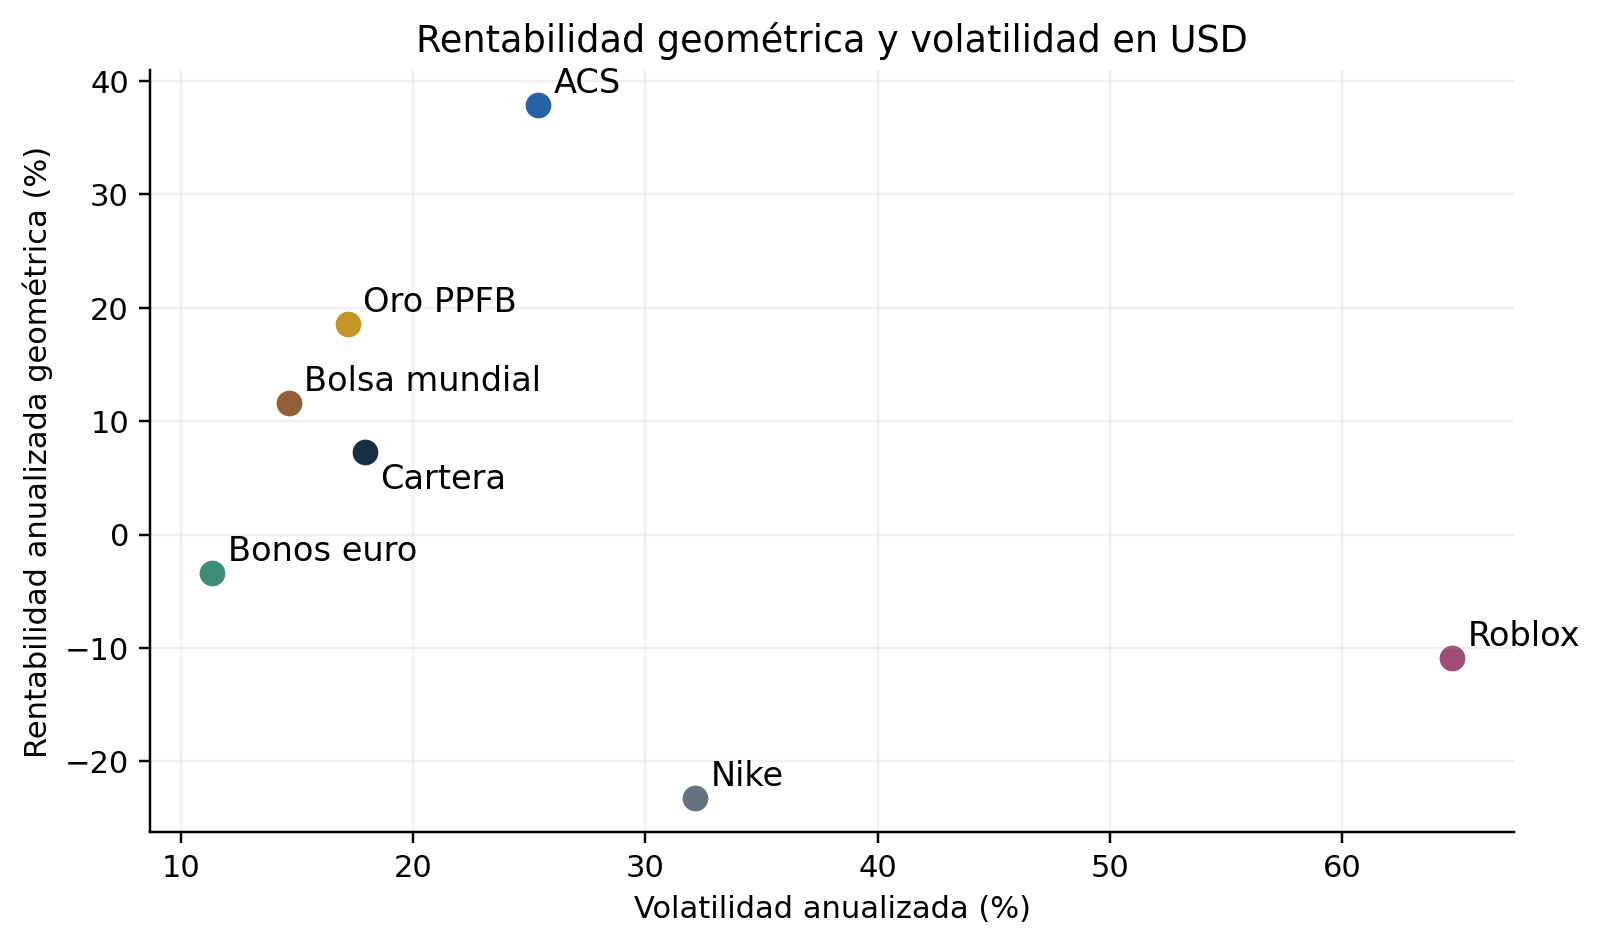
\includegraphics[width=1.000\linewidth,keepaspectratio]{../figures/risk_return_usd.png}
\captionof{figure}[Rentabilidad y volatilidad]{Volatilidad anualizada y rentabilidad anualizada geométrica en USD.}
\label{fig:risk_return}
\end{figure}\par
La volatilidad resume el riesgo total observado. Este gráfico es descriptivo. La SML relaciona la rentabilidad esperada con beta, que mide la sensibilidad al mercado.

\Needspace{7\baselineskip}\subsection{Diversificación y contraste en euros}
En la figura~\ref{fig:correlations}, la correlación de Bolsa mundial con Oro PPFB es 0,2989 y con Bonos euro, 0,6875.
En esta muestra, el oro se movió menos en sintonía con la bolsa mundial que los bonos soberanos de la zona euro. Esa menor correlación favorece la diversificación frente al riesgo bursátil. El efecto sobre el riesgo total también depende de los pesos y las volatilidades.

Los pesos iguales en capital no implican contribuciones iguales al riesgo.

\par\begin{figure}[!htbp]\centering
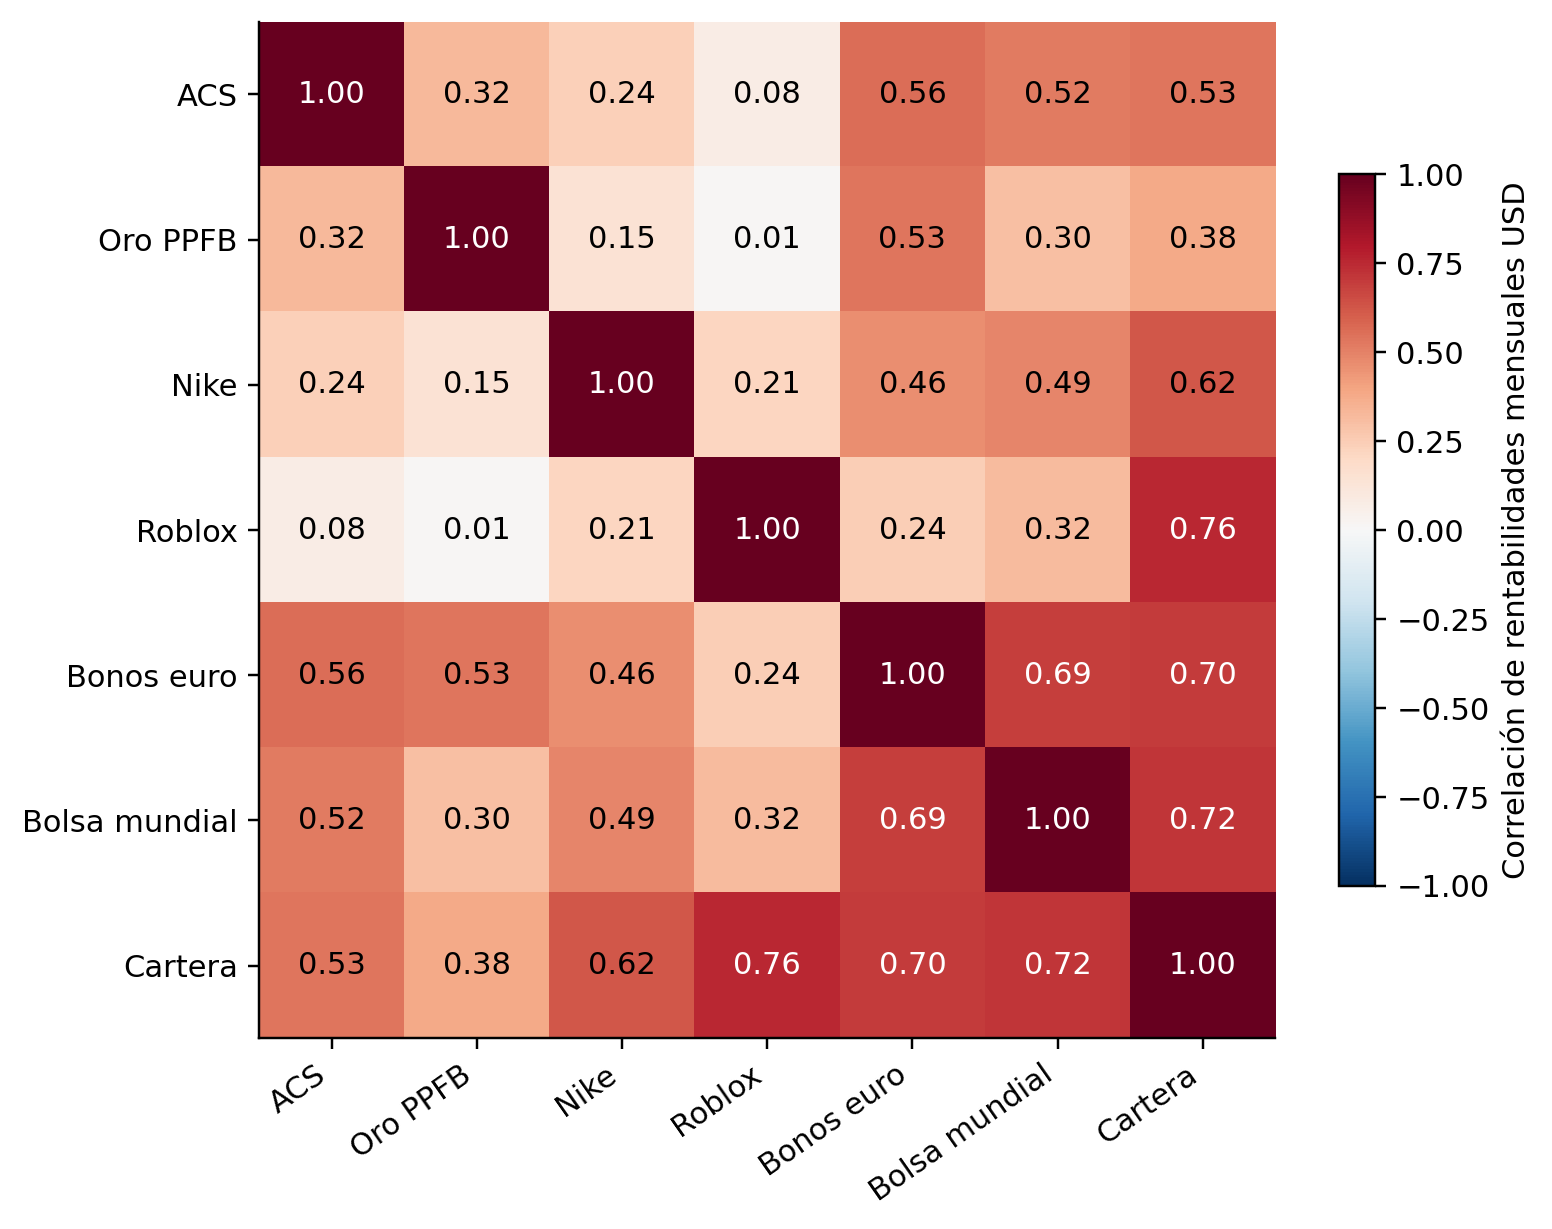
\includegraphics[width=0.837\linewidth,keepaspectratio]{../figures/correlations_usd.png}
\captionof{figure}[Correlaciones mensuales]{Correlaciones de Pearson en los 60 meses comunes, en USD.}
\label{fig:correlations}
\end{figure}\par
Cada activo forma parte de la cartera, por lo que su propia rentabilidad contribuye a la correlación que observamos entre ambos. Las correlaciones pueden cambiar fuera de la muestra. Incluso los activos poco ligados a la bolsa están expuestos a riesgos como los tipos de interés, el crédito, las materias primas o la divisa.

\par\noindent\begin{minipage}{\linewidth}
\captionof{table}[Rentabilidad y riesgo en EUR]{Rentabilidad y riesgo en EUR}
\label{tab:descriptive-eur}
\begingroup\small
\begin{tabular}{L{\dimexpr 0.30612\linewidth-2\tabcolsep\relax}R{\dimexpr 0.23469\linewidth-2\tabcolsep\relax}R{\dimexpr 0.22449\linewidth-2\tabcolsep\relax}R{\dimexpr 0.23469\linewidth-2\tabcolsep\relax}}
\toprule
\rowcolor{light} \textbf{Activo} & \textbf{Geom anual EUR} & \textbf{Vol anual EUR} & \textbf{Acumulada EUR} \\
\midrule
ACS & 38,53 \% & 22,30 \% & 410,18 \% \\
Oro PPFB & 19,09 \% & 14,58 \% & 139,56 \% \\
Nike & -22,85 \% & 30,06 \% & -72,67 \% \\
Roblox & -10,52 \% & 65,64 \% & -42,63 \% \\
Bonos euro & -2,98 \% & 6,60 \% & -14,04 \% \\
Bolsa mundial & 12,08 \% & 12,78 \% & 76,89 \% \\
\midrule
Cartera & 7,80 \% & 15,88 \% & 45,59 \% \\
\bottomrule
\end{tabular}
\endgroup
\par\medskip
\end{minipage}\par\medskip
Para el cálculo en euros aplicamos los mismos pesos a las rentabilidades en EUR. Cada activo conserva su fecha efectiva de cierre. Las regresiones se estiman en USD.

La volatilidad anualizada de Bonos euro es 11,35 \% en USD y 6,60 \% en EUR. La diferencia muestra que la moneda influye en el riesgo observado, sin aislar una contribución causal del cambio.

\Needspace{7\baselineskip}\section{CAPM por activo}
En el CAPM teórico, la beta mide la exposición al riesgo de mercado y determina la prima de rentabilidad esperada del activo.

\[E(R_i)=R_f+\beta_i[E(R_M)-R_f].\]
En la aplicación empírica se estima por mínimos cuadrados ordinarios (OLS) una regresión con intercepto sobre 60 excesos de rentabilidad mensuales comunes a los activos y a la cartera.

\[R_{i,t}-R_{f,t}=\alpha_i+\beta_i(R_{M,t}-R_{f,t})+\varepsilon_{i,t}.\]
El contraste \(H_0:\alpha_i=0\) evalúa si la rentabilidad media difiere de la indicada por la referencia CAPM. El contraste \(H_0:\beta_i=0\) evalúa la sensibilidad lineal al mercado. Ambos se realizan al 5 \% nominal. La significación de beta acredita sensibilidad al factor. Un alfa compatible con cero indica que los datos son compatibles con esa implicación del modelo. La validez general del CAPM requiere evidencia adicional. La inferencia convencional supone homocedasticidad y ausencia de autocorrelación.
La tabla~\ref{tab:capm} resume la sensibilidad al mercado y el alfa mensual por activo y para la cartera.
\par\noindent\begin{minipage}{\linewidth}
\captionof{table}[CAPM por activo y cartera (OLS)]{CAPM por activo y cartera (OLS)}
\label{tab:capm}
\begingroup\small
\begin{tabular}{L{\dimexpr 0.21429\linewidth-2\tabcolsep\relax}R{\dimexpr 0.14082\linewidth-2\tabcolsep\relax}R{\dimexpr 0.12857\linewidth-2\tabcolsep\relax}R{\dimexpr 0.12857\linewidth-2\tabcolsep\relax}R{\dimexpr 0.12857\linewidth-2\tabcolsep\relax}R{\dimexpr 0.12857\linewidth-2\tabcolsep\relax}R{\dimexpr 0.13061\linewidth-2\tabcolsep\relax}}
\toprule
\rowcolor{light} \textbf{Activo} & \textbf{Alfa mes} & \textbf{p alfa} & \textbf{Beta} & \textbf{p beta} & \textbf{R\textsuperscript{2}} & \textbf{R\textsuperscript{2} ajustado} \\
\midrule
ACS & 2,12 \% & 0,0176 & 0,6964 & 0,0005 & 0,1917 & 0,1778 \\
Oro PPFB & 1,11 \% & 0,0896 & 0,1649 & 0,2423 & 0,0235 & 0,0067 \\
Nike & -2,87 \% & 0,0082 & 1,0436 & <0,0001 & 0,2673 & 0,2547 \\
Roblox & -0,73 \% & 0,7523 & 1,5136 & 0,0034 & 0,1386 & 0,1237 \\
Bonos euro & -0,89 \% & 0,0102 & 0,4376 & <0,0001 & 0,3874 & 0,3768 \\
Bolsa mundial & 0,01 \% & 0,9681 & 0,8769 & <0,0001 & 0,9210 & 0,9197 \\
\midrule
Cartera & -0,21 \% & 0,6691 & 0,7888 & <0,0001 & 0,4969 & 0,4882 \\
\bottomrule
\end{tabular}
\endgroup
\par\medskip
\end{minipage}\par\medskip
Alfa positivo y significativo al 5 \% con OLS en ACS.

Alfa negativo y significativo al 5 \% con OLS en Nike, Bonos euro.

Entre los activos, el R\textsuperscript{2} va de 0,0235 en Oro PPFB a 0,9210 en Bolsa mundial.

La beta de la cartera es 0,7888. Un aumento de un punto porcentual en el exceso mensual del mercado se asocia con un cambio estimado de 0,79 puntos porcentuales en el exceso de la cartera.

Roblox presenta la mayor beta entre los activos (1,5136). La volatilidad resume el riesgo total observado. La beta mide sensibilidad al mercado y el R\textsuperscript{2}, la proporción de variación del exceso de rentabilidad que recoge el modelo. El residuo puede incluir riesgo específico y riesgos comunes omitidos. La diversificación tiende a reducir el componente específico.

Para Oro PPFB, la beta estimada es 0,1649 (p = 0,2423). La evidencia de sensibilidad lineal al mercado es insuficiente al 5 \%. El oro sigue expuesto a riesgos propios de precio y divisa.

\Needspace{6\baselineskip}\[\widehat\beta_p=\sum_{i=1}^{6}w_i\widehat\beta_i.\]
Al ponderar las betas individuales se obtiene 0,7888, que coincide hasta el redondeo con la estimación directa de la cartera. La igualdad se deriva de la linealidad de OLS con pesos constantes que suman uno y regresiones con intercepto sobre los mismos meses, moneda, RF y factor de mercado.

\Needspace{7\baselineskip}\subsection{SML estimada con medias históricas}
\begin{equation*}
\overline R_i^{\mathrm{SML}}=\overline{\mathrm{RF}}+\widehat\beta_i\,\overline{\mathrm{Mkt-RF}},\qquad \overline R_i-\overline R_i^{\mathrm{SML}}=\widehat\alpha_i.
\end{equation*}
En la figura~\ref{fig:sml}, la distancia vertical entre cada punto y la recta mide el alfa de Jensen mensual respecto a la referencia utilizada.
\par\begin{figure}[!htbp]\centering
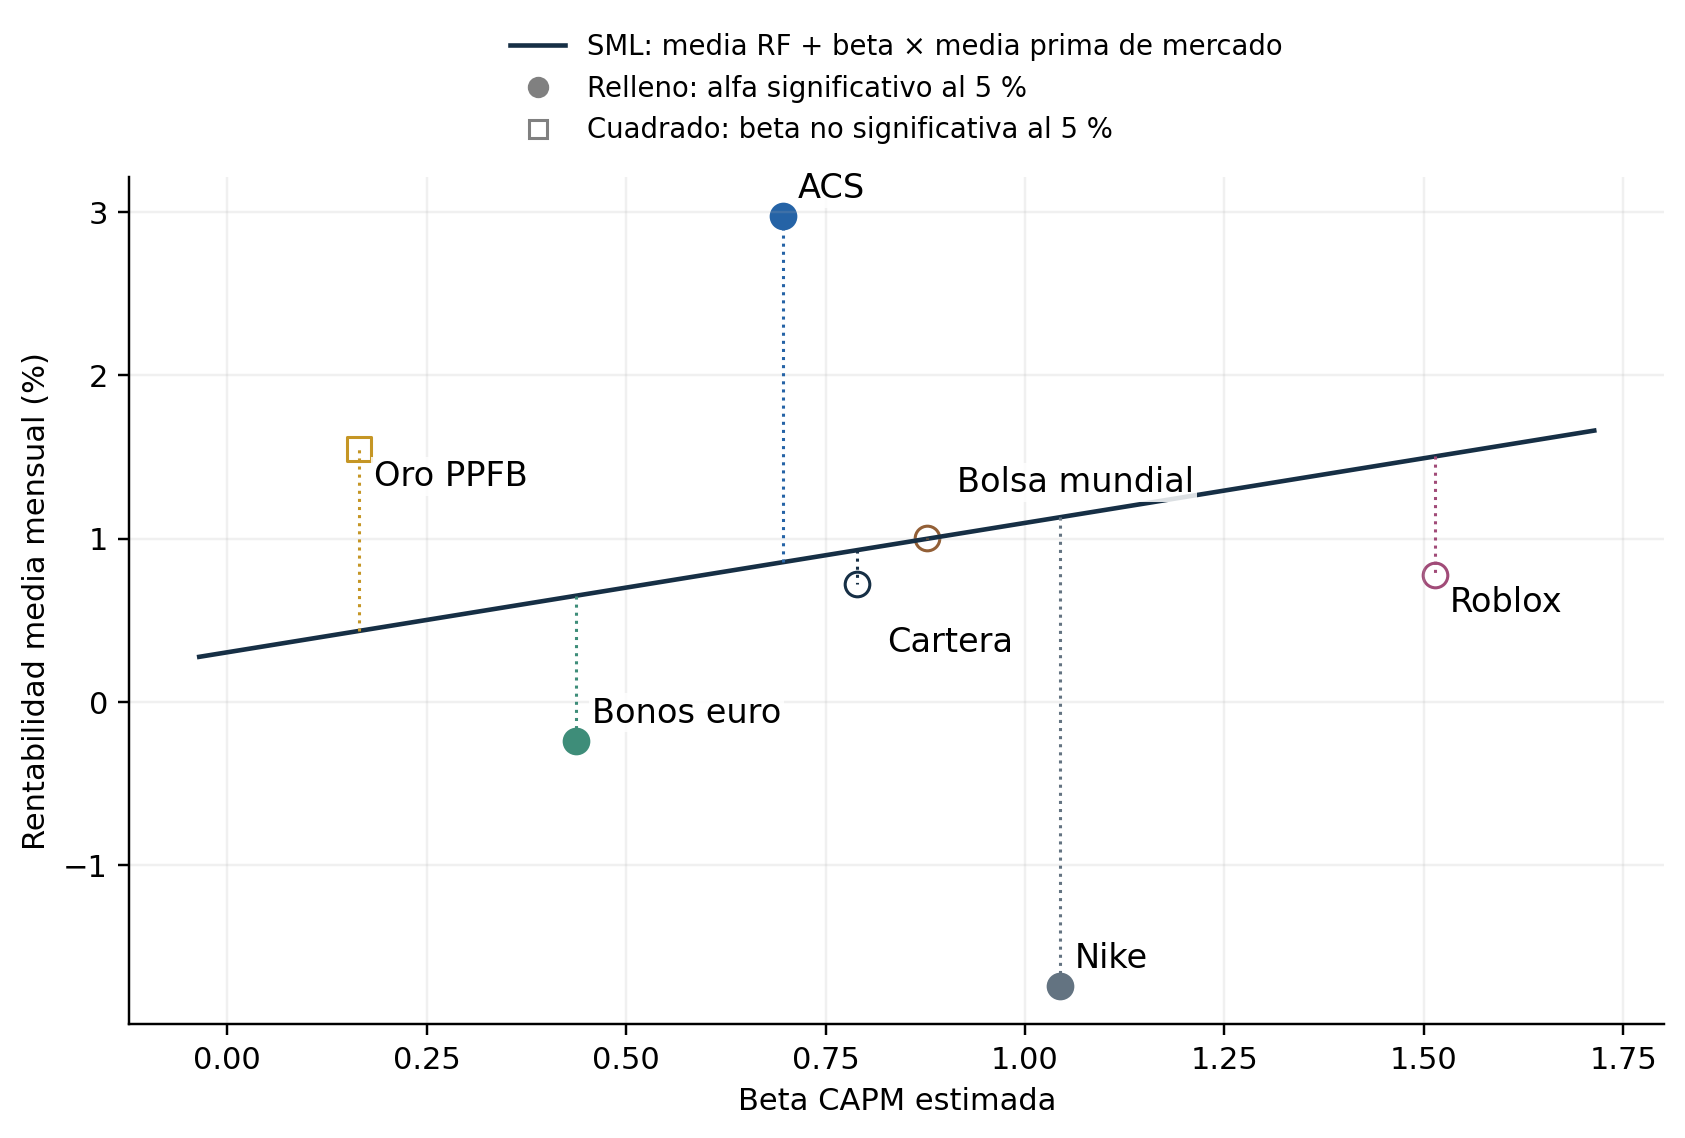
\includegraphics[width=1.000\linewidth,keepaspectratio]{../figures/sml_usd.png}
\captionof{figure}[SML histórica]{SML estimada con medias históricas mensuales en USD.}
\label{fig:sml}
\end{figure}\par
Para cada beta, la recta suma la media de RF y la prima media de mercado multiplicada por esa beta. Los puntos muestran las rentabilidades medias observadas en los mismos meses y en USD. Los puntos rellenos señalan alfas significativos y los cuadrados, betas no significativas al 5 \% con OLS.

ACS queda por encima de la SML, y Nike y Bonos euro por debajo, con alfas OLS significativos. Las distancias reflejan rendimiento medio no recogido por la referencia del CAPM en estos meses. La elección de la referencia y los riesgos omitidos limitan la atribución de estos alfas a la habilidad de gestión.

\Needspace{7\baselineskip}\section{Cartera y Fama--French de tres factores}
\begin{equation*}
R_{p,t}-\mathrm{RF}_t=\alpha_p+\beta_m(\mathrm{Mkt-RF})_t+\beta_s\,\mathrm{SMB}_t+\beta_h\,\mathrm{HML}_t+\varepsilon_{p,t}.
\end{equation*}
En la tabla~\ref{tab:ff3}, el alfa, su error estándar y su intervalo se expresan en porcentaje mensual. Las exposiciones y sus errores e intervalos son adimensionales.
\par\noindent\begin{minipage}{\linewidth}
\captionof{table}[Coeficientes FF3 de la cartera (OLS)]{Coeficientes FF3 de la cartera (OLS)}
\label{tab:ff3}
\begingroup\small
\begin{tabular}{L{\dimexpr 0.16327\linewidth-2\tabcolsep\relax}R{\dimexpr 0.15306\linewidth-2\tabcolsep\relax}R{\dimexpr 0.14286\linewidth-2\tabcolsep\relax}R{\dimexpr 0.12245\linewidth-2\tabcolsep\relax}R{\dimexpr 0.12245\linewidth-2\tabcolsep\relax}R{\dimexpr 0.14694\linewidth-2\tabcolsep\relax}R{\dimexpr 0.14898\linewidth-2\tabcolsep\relax}}
\toprule
\rowcolor{light} \textbf{Término} & \textbf{Estimación} & \textbf{Error est} & \textbf{t} & \textbf{p} & \textbf{IC95 inf} & \textbf{IC95 sup} \\
\midrule
alpha & -0,04 \% & 0,50 \% & -0,0709 & 0,9437 & -1,05 \% & 0,98 \% \\
Mkt-RF & 0,7425 & 0,1114 & 6,6642 & <0,0001 & 0,5193 & 0,9657 \\
SMB & 0,1369 & 0,1817 & 0,7532 & 0,4545 & -0,2271 & 0,5009 \\
HML & -0,1375 & 0,1269 & -1,0835 & 0,2832 & -0,3916 & 0,1167 \\
\bottomrule
\end{tabular}
\endgroup
\par\medskip
\end{minipage}\par\medskip
SMB mide la diferencia de rentabilidad entre carteras de empresas pequeñas y grandes. HML mide la diferencia entre carteras con un cociente valor contable sobre valor de mercado alto y bajo, respectivamente. Cada exposición mide la sensibilidad al factor manteniendo constantes los demás. Los pesos de capital se fijan al construir la cartera.

\par\noindent\begin{minipage}{\linewidth}
\captionof{table}[Comparación CAPM y FF3]{Comparación CAPM y FF3}
\label{tab:comparison}
\begingroup\small
\begin{tabular}{L{\dimexpr 0.18367\linewidth-2\tabcolsep\relax}R{\dimexpr 0.10204\linewidth-2\tabcolsep\relax}R{\dimexpr 0.16327\linewidth-2\tabcolsep\relax}R{\dimexpr 0.20408\linewidth-2\tabcolsep\relax}R{\dimexpr 0.17347\linewidth-2\tabcolsep\relax}R{\dimexpr 0.17347\linewidth-2\tabcolsep\relax}}
\toprule
\rowcolor{light} \textbf{Modelo} & \textbf{N} & \textbf{R\textsuperscript{2}} & \textbf{R\textsuperscript{2} ajustado} & \textbf{AIC} & \textbf{BIC} \\
\midrule
CAPM & 60 & 0,4969 & 0,4882 & -224,11 & -219,92 \\
FF3 & 60 & 0,5110 & 0,4848 & -221,82 & -213,44 \\
\bottomrule
\end{tabular}
\endgroup
\par\medskip
\end{minipage}\par\medskip
Los signos estimados apuntan a una exposición positiva al diferencial de pequeñas frente a grandes y negativa al diferencial de valor. Ambos intervalos de confianza incluyen cero, por lo que la evidencia individual al 5 \% es insuficiente para atribuir a la cartera una orientación por tamaño o estilo.

Los valores p de SMB (0,4545) y HML (0,2832) corresponden a contrastes individuales. La comparación utiliza las mismas observaciones en ambos modelos.

Al añadir SMB y HML, el R\textsuperscript{2} ajustado baja: pasa de 0,4882 en el CAPM a 0,4848 en FF3. Esta medida penaliza el número de regresores y describe el ajuste dentro de la muestra.

El contraste conjunto evalúa \(H_0:\beta_{\mathrm{SMB}}=\beta_{\mathrm{HML}}=0\).
El contraste da F(2, 56) = 0,8099 y p = 0,4500. Al 5 \%, no se rechaza la hipótesis nula bajo los supuestos de la inferencia OLS convencional.

La sensibilidad Newey–West \cite{nw} se recoge en las tablas~\ref{tab:hac-capm} y~\ref{tab:hac-ff3}.
La estimación HAC usa 3 retardos. HAC mantiene la clasificación nominal de los alfas CAPM al 5 \%.

En ACS, el valor p pasa de 0,0176 a 0,0450 y queda cerca del umbral. La muestra y la multiplicidad de contrastes limitan la inferencia.

\Needspace{7\baselineskip}\section{Limitaciones y conclusiones}
La prima de mercado de EE. UU. tiene una capacidad explicativa distinta según el activo. El CAPM recoge el 92,10 \% de la variación mensual del exceso de rentabilidad de Bolsa mundial y el 2,35 \% en Oro PPFB.

El ajuste de IUSQ es coherente con que la renta variable mundial y la estadounidense compartan movimientos bursátiles. En el oro queda casi toda la variación por explicar. Los tipos reales y el dólar son canales plausibles, aunque estas regresiones solo estiman la relación con la prima bursátil.

La beta de la cartera es 0,7888. Un aumento de un punto porcentual en la prima mensual de mercado se asocia con un cambio estimado de 0,79 puntos porcentuales en el exceso de rentabilidad de la cartera. El alfa mensual es -0,21 \% con CAPM (p = 0,6691) y -0,04 \% con FF3 (p = 0,9437). Ambas estimaciones son compatibles con un alfa nulo al 5 \%.

Al incorporar tamaño y valor, el R\textsuperscript{2} bruto pasa de 0,4969 a 0,5110 y el ajustado pasa de 0,4882 a 0,4848. AIC y BIC también favorecen el CAPM. Con p = 0,4500, al 5 \% no se rechaza que ambos coeficientes sean cero bajo los supuestos de OLS convencional. Para describir esta cartera en la muestra, la evidencia favorece el CAPM como especificación más sencilla.

Las conclusiones corresponden a 60 meses y a una referencia bursátil estadounidense, que recoge de forma parcial los riesgos de tipos, divisas y materias primas. Los precios pueden revisarse y los cierres de los activos y del mercado de divisas ocurren a horas distintas.

\Needspace{7\baselineskip}\section{Disponibilidad de datos y reproducibilidad}
El código de Python genera las estimaciones y las figuras a partir de las series mensuales. El repositorio reúne las estimaciones, las estadísticas descriptivas y las correlaciones agregadas. El libro adjunto a la entrega académica contiene los datos mensuales, los pesos, las fórmulas de conversión y rentabilidad y las regresiones exportadas. Regenerar las estimaciones requiere ejecutar el código con los insumos originales.

La \href{https://github.com/jaimeeblancoo/beyond-beta/blob/main/docs/reviewer_guide.md}{guía de verificación} enlaza cada resultado con su cálculo y explica cómo ejecutar el código con datos sintéticos o con insumos propios autorizados.

\Needspace{14\baselineskip}\section{Referencias y fuentes}
\begingroup\small\setlength{\parskip}{4pt}
\begingroup\renewcommand{\section}[2]{}\begin{thebibliography}{9}
\bibitem{sharpe} Sharpe, W. F. (1964). Capital asset prices: A theory of market equilibrium under conditions of risk. \textit{The Journal of Finance}, 19(3), 425--442. \href{https://doi.org/10.1111/j.1540-6261.1964.tb02865.x}{DOI}.
\bibitem{ff} Fama, E. F., y French, K. R. (1993). Common risk factors in the returns on stocks and bonds. \textit{Journal of Financial Economics}, 33(1), 3--56. \href{https://doi.org/10.1016/0304-405X(93)90023-5}{DOI}.
\bibitem{nw} Newey, W. K., y West, K. D. (1987). A simple, positive semi-definite, heteroskedasticity and autocorrelation consistent covariance matrix. \textit{Econometrica}, 55(3), 703--708. \href{https://doi.org/10.2307/1913610}{DOI}.
\bibitem{factors} French, K. R. (2026). \textit{Description of Fama/French factors}. Data Library. Copia mensual CRSP 202609. \href{https://mba.tuck.dartmouth.edu/pages/faculty/ken.french/data_library/f-f_factors.html}{Biblioteca de datos}.
\bibitem{yahoo} Yahoo Finance (2026). \textit{Historical data}. Series ACS.MC, PPFB.DE, NKE, RBLX, EUNH.DE, IUSQ.DE y EURUSD=X, obtenidas mediante yfinance. \href{https://finance.yahoo.com/}{Históricos}. \href{https://ranaroussi.github.io/yfinance/reference/api/yfinance.download.html}{Documentación de yfinance}.
\bibitem{ishares} BlackRock/iShares (2026). \textit{Fichas de productos}. iShares Physical Gold ETC, ISIN IE00B4ND3602, \href{https://www.ishares.com/gls-download/literature/fact-sheet/sgln-ishares-physical-gold-etc-fund-fact-sheet-en-de.pdf}{ficha PPFB}. iShares Core Euro Government Bond UCITS ETF, ISIN IE00B4WXJJ64: \href{https://www.ishares.com/gls-download/literature/fact-sheet/iega-ishares-core-govt-bond-ucits-etf-fund-fact-sheet-en-de.pdf}{Ficha EUNH}. iShares MSCI All Country World UCITS ETF, ISIN IE00B6R52259: \href{https://www.ishares.com/uk/individual/en/products/251850/ishares-msci-acwi-ucits-etf}{Ficha IUSQ}.
\end{thebibliography}\endgroup
\endgroup
\clearpage
\appendix
\section{Resultados completos del CAPM}
El porcentaje mensual facilita la comparación de los alfas, sus errores estándar e intervalos con las tablas del cuerpo. Las betas y su incertidumbre se expresan en unidades adimensionales.

\par\noindent\begin{minipage}{\linewidth}
\captionof{table}[Coeficientes CAPM completos (OLS)]{Coeficientes CAPM completos (OLS)}
\label{tab:capm-full}
\begingroup\small
\begin{tabular}{L{\dimexpr 0.26122\linewidth-2\tabcolsep\relax}R{\dimexpr 0.13265\linewidth-2\tabcolsep\relax}R{\dimexpr 0.13265\linewidth-2\tabcolsep\relax}R{\dimexpr 0.10612\linewidth-2\tabcolsep\relax}R{\dimexpr 0.10612\linewidth-2\tabcolsep\relax}R{\dimexpr 0.13061\linewidth-2\tabcolsep\relax}R{\dimexpr 0.13061\linewidth-2\tabcolsep\relax}}
\toprule
\rowcolor{light} \textbf{Activo y término} & \textbf{Coef.} & \textbf{Error est} & \textbf{t} & \textbf{p} & \textbf{IC95 inf} & \textbf{IC95 sup} \\
\midrule
ACS alpha & 2,12 \% & 0,87 \% & 2,4437 & 0,0176 & 0,38 \% & 3,86 \% \\
ACS Mkt-RF & 0,6964 & 0,1877 & 3,7091 & 0,0005 & 0,3206 & 1,0722 \\
Oro PPFB alpha & 1,11 \% & 0,65 \% & 1,7267 & 0,0896 & -0,18 \% & 2,41 \% \\
Oro PPFB Mkt-RF & 0,1649 & 0,1396 & 1,1814 & 0,2423 & -0,1145 & 0,4443 \\
Nike alpha & -2,87 \% & 1,05 \% & -2,7367 & 0,0082 & -4,97 \% & -0,77 \% \\
Nike Mkt-RF & 1,0436 & 0,2268 & 4,6002 & <0,0001 & 0,5895 & 1,4977 \\
Roblox alpha & -0,73 \% & 2,29 \% & -0,3170 & 0,7523 & -5,31 \% & 3,86 \% \\
Roblox Mkt-RF & 1,5136 & 0,4955 & 3,0547 & 0,0034 & 0,5218 & 2,5054 \\
Bonos euro alpha & -0,89 \% & 0,33 \% & -2,6553 & 0,0102 & -1,56 \% & -0,22 \% \\
Bonos euro Mkt-RF & 0,4376 & 0,0723 & 6,0561 & <0,0001 & 0,2930 & 0,5823 \\
Bolsa mundial alpha & 0,01 \% & 0,16 \% & 0,0402 & 0,9681 & -0,31 \% & 0,32 \% \\
Bolsa mundial Mkt-RF & 0,8769 & 0,0337 & 26,0058 & <0,0001 & 0,8094 & 0,9444 \\
Cartera alpha & -0,21 \% & 0,48 \% & -0,4296 & 0,6691 & -1,17 \% & 0,76 \% \\
Cartera Mkt-RF & 0,7888 & 0,1042 & 7,5681 & <0,0001 & 0,5802 & 0,9974 \\
\bottomrule
\end{tabular}
\endgroup
\par\medskip
\end{minipage}\par\medskip
Se estiman 7 CAPM y un FF3, todos con intercepto y 60 meses. Los errores y resultados HAC completos están disponibles en las tablas agregadas del repositorio.

\Needspace{7\baselineskip}
\clearpage
\section{Sensibilidad de la inferencia}
Los residuos mensuales pueden presentar heterocedasticidad o dependencia temporal. Como comprobación, se estima la covarianza HAC con ponderaciones de Bartlett y 3 retardos. La corrección afecta a errores estándar, valores p e intervalos. Con 60 meses, la inferencia robusta sigue siendo aproximada y el contraste conjunto anterior conserva su alcance convencional.

\par\noindent\begin{minipage}{\linewidth}
\captionof{table}[Sensibilidad de los alfas CAPM (HAC)]{Sensibilidad de los alfas CAPM (HAC)}
\label{tab:hac-capm}
\begingroup\small
\begin{tabular}{L{\dimexpr 0.26531\linewidth-2\tabcolsep\relax}R{\dimexpr 0.16327\linewidth-2\tabcolsep\relax}R{\dimexpr 0.16327\linewidth-2\tabcolsep\relax}R{\dimexpr 0.20408\linewidth-2\tabcolsep\relax}R{\dimexpr 0.20408\linewidth-2\tabcolsep\relax}}
\toprule
\rowcolor{light} \textbf{CAPM} & \textbf{p alfa OLS} & \textbf{p alfa HAC} & \textbf{IC95 HAC inf} & \textbf{IC95 HAC sup} \\
\midrule
ACS & 0,0176 & 0,0450 & 0,05 \% & 4,19 \% \\
Oro PPFB & 0,0896 & 0,1164 & -0,29 \% & 2,51 \% \\
Nike & 0,0082 & 0,0029 & -4,72 \% & -1,02 \% \\
Roblox & 0,7523 & 0,7570 & -5,40 \% & 3,95 \% \\
Bonos euro & 0,0102 & 0,0197 & -1,63 \% & -0,15 \% \\
Bolsa mundial & 0,9681 & 0,9636 & -0,27 \% & 0,28 \% \\
\midrule
Cartera & 0,6691 & 0,7158 & -1,34 \% & 0,93 \% \\
\bottomrule
\end{tabular}
\endgroup
\par\medskip
\end{minipage}\par\medskip
En FF3, el error estándar y el intervalo del alfa se expresan en porcentaje mensual.

\par\noindent\begin{minipage}{\linewidth}
\captionof{table}[Inferencia HAC de la cartera FF3]{Inferencia HAC de la cartera FF3}
\label{tab:hac-ff3}
\begingroup\small
\begin{tabular}{L{\dimexpr 0.18367\linewidth-2\tabcolsep\relax}R{\dimexpr 0.16327\linewidth-2\tabcolsep\relax}R{\dimexpr 0.14286\linewidth-2\tabcolsep\relax}R{\dimexpr 0.14286\linewidth-2\tabcolsep\relax}R{\dimexpr 0.18367\linewidth-2\tabcolsep\relax}R{\dimexpr 0.18367\linewidth-2\tabcolsep\relax}}
\toprule
\rowcolor{light} \textbf{FF3 término} & \textbf{Error HAC} & \textbf{t HAC} & \textbf{p HAC} & \textbf{IC95 inferior} & \textbf{IC95 superior} \\
\midrule
alpha & 0,56 \% & -0,0640 & 0,9492 & -1,16 \% & 1,08 \% \\
Mkt-RF & 0,0877 & 8,4646 & <0,0001 & 0,5668 & 0,9182 \\
SMB & 0,1807 & 0,7574 & 0,4520 & -0,2251 & 0,4989 \\
HML & 0,1183 & -1,1618 & 0,2503 & -0,3745 & 0,0996 \\
\bottomrule
\end{tabular}
\endgroup
\par\medskip
\end{minipage}\par\medskip
\Needspace{7\baselineskip}
\end{document}
